\chapter{Escenario de trabajo. Descripción y requisitos.}\label{sec:EscenarioTrabajo}

\paragraph{}En este capítulo se presenta al equipo ficticio de desarrollo, se habla
de sus necesidades y de cómo van a interactuar con el entorno. Si consideramos a los
desarrolladores como nuestros clientes o usuarios, podemos aplicar técnicas de análisis
de sus necesidades tales como \textit{Customer Personas} (figura \ref{fig:customer_persona})
o Mapas de Empatía (figura \ref{fig:mapa_empatia}). Estás técnicas son muy comunes
dentro de departamentos de Marketing, su uso garantiza que el diseño del producto se
hará entorno a las necesidades de los clientes, en este caso, del entorno de desarrollo
y los propios desarrolladores. En nuestra versión, vamos a agrupar a los usuarios por
\textit{expertise} y vamos a definir necesidades para equipos.

\begin{figure}[ht]
    \centering
    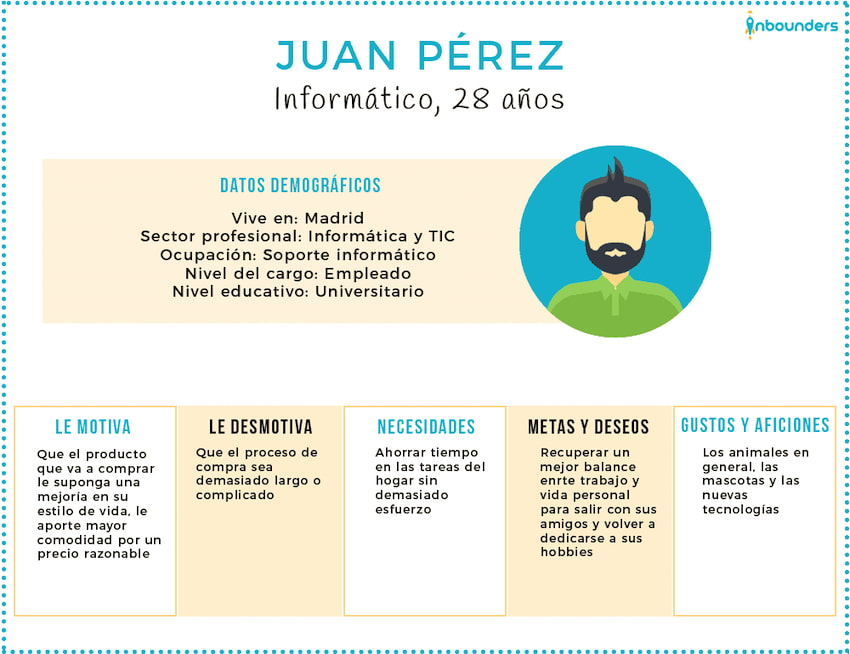
\includegraphics[width=0.65\textwidth]{imgs/buyer-persona-ejemplo.jpg}
    \caption{Ejemplo \textit{Customer Persona} utilizado en Marketing}
    \label{fig:customer_persona}
\end{figure}

\begin{figure}[H]
    \centering
    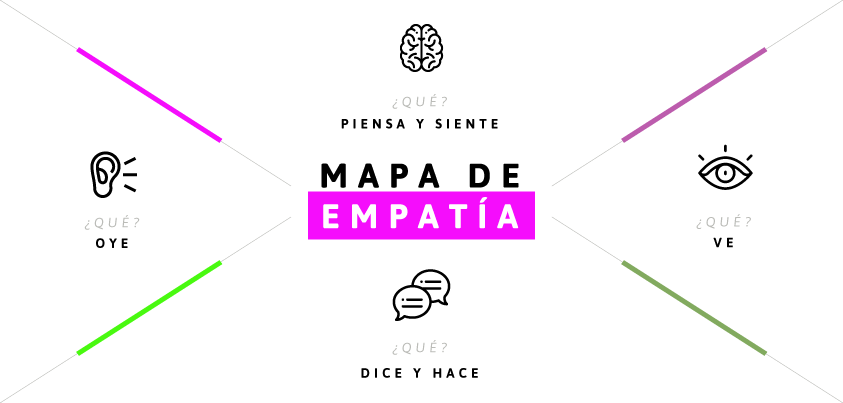
\includegraphics[width=0.65\textwidth]{imgs/mapa-empatia.png}
    \caption{Esquema resumen del Mapa de Empatía utilizado en Marketing}
    \label{fig:mapa_empatia}
\end{figure}

\section{Equipo de desarrollo de software de sistema}\label{sec:systemteam}

\paragraph{}La gran mayoría de productos de \gls{IoT} basados en microprocesadores,
tienen un sistema operativo sobre el cual se ejecutan las aplicaciones, servicios o
microservicios. Los desarrolladores del software de sistema se encargan de gestionar
este sistema operativo. Los principales aspectos que deben tener en cuenta son:

\begin{itemize}
    \item Proveer de las librerías necesarias para la ejecución de la aplicaciones o
    servicios.
    \item Velar por la estabilidad del sistema.
    \item Asegurar la ciberseguridad del dispositivo.
    \item Proveer el acceso a los recursos hardware por parte del software, mediante
    drivers propios o desarrollados por terceros.
    \item En muchos caso, desarrollan las herramientas de distribuición y despliegue
    de todo el software en los dispositivos.
\end{itemize}

\paragraph{}La principales herramientas de trabajo dentro del entorno de desarrollo para este equipo
será:

\begin{itemize}
    \item Yocto \ref{sec:yocto} y bitbake para el desarrollo de layers \ref{layers} y
    recipes \ref{recipes}.
    \item Uso de la consola o \gls{shell}.
    \item Lenguaje de programación Bash, para el desarrollo de \gls{scripts} que se
    ejecutan en la consola.
    \item Lenguaje de programación Python, para el desarrollo de \gls{scripts} más complejos.
    \item Programa de edición de texto para la edición de los ficheros, será recomendable
    el uso de \hyperref[sec:vscode]{Visual Studio Code} como \gls{IDE}.
\end{itemize}

\section{Equipo de desarrollado de aplicaciones UI/UX}\label{sec:uiteam}

\paragraph{}El equipo de \gls{UI/UX} se dedica como su propio nombre indica a la interfaz
de usuario y a la interacción con la misma. Dicho de otra manera, el equipo de \gls{UI/UX}
están a cargo del desarrollo del \gls{front-end}. Su objetivo es crear una interfaz
alineada con las necesidades del usuario medio al que destinada, así como, generar una
experiencia adecuada de uso. Es importante que la interfaz represente los objetivos de
negocio, ya que es la principal conexión con el usuario y por tanto la mayor fuente de
percepción de información y de imagen de marca.

\paragraph{}Técnicamente, la interfaz debe tener en cuenta las expecificaciones de diseño,
los requisitos, el uso de recursos de cálculo así como los recursos del \gls{SDK}
utilizado para el desarrollo.

\paragraph{}El desarrollo de la interfaz suele ser independiente al desarrollo de la
lógica de los servicios, permitiendo así la autogestión de los equipos de desarrollo.
Sin embargo, para las labores de testing en frecuente necesitar ambas partes para
comprobar que la interfaz se comporta de manera coherente con la lógica. Por eso, el
entorno de desarrollo debe permitir el desarrollo de manera independiente de la interfaz
y la ejecución de ambas maneras, tanto independiente en conjunto con el \gls{back-end}.

\paragraph{}Los principales aspectos que deben tener en cuenta son:

\begin{itemize}
    \item Ejecución independiente de la interfaz.
    \item Ejecución conjunta con el \gls{back-end}.
\end{itemize}

\paragraph{}La principales herramientas de trabajo dentro del entorno de desarrollo para este equipo
será:

\begin{itemize}
    \item \hyperref[sec:vscode]{Visual Studio Code} como \gls{IDE}.
    \item Lenguaje de programación Flutter/Dart.
\end{itemize}

\section{Equipo de desarrollo de servicios de aplicaciones}

\paragraph{}También conocido como el equipo de \gls{back-end} es el encargado de programar
la lógica del programa. También suelen programar la comunicación con dispositivos externos,
ya sean dispositivos hardware como dispositivos de red. Suelen estar en permanente
contacto con el \hyperref[sec:uiteam]{equipo de UI/UX} para coordinar la representación
de los distintos datos en la interfaces visuales, de la misma manera, están en contacto
con el \hyperref[sec:systemteam]{equipo de software de sistema} para concretar los
recursos, métodos y protocolos disponibles para hacer llamadas, peticiones o contestar
a llamadas, peticiones y eventos externos.

\paragraph{}Tienen una gran responsabilidad al hacer de ``puente'' entre el resto de
equipos, suelen tener a los programadores con mejores \emph{skills} técnicas. Los
lenguajes de programación más utilizados son C/C++, Rust, Go o Dart por citar unos pocos.
En este caso, la aplicación tiene una arquitectura monolítica, que en contra posición
con la tendencia de microservicios actual, concentra todo el código en un sólo fichero
binario ejecutable. Aunque una arquitectura monolítica puede utilizar diferentes hilos
de ejecución, desde el punto de vista del sistema operativo toda la aplicación es un
mismo servicio en ejecución.

\section{Equipo de integración y distribución DevOps}

\paragraph{}Blabla

\section{Equipo de testing y QA}

\paragraph{}Blabla

%las referencias a artículos se ponen con \cite,
%las referencias a glosario \gls,
%y las referencias a ecuaciones \eqref
%las referencias a imgenes, tablas o figuras o secciones
% se ponen con \ref (sólo número) o con \hyperref[sec:X]{Blabla}